\documentclass[a4paper]{assignment}

\coursetitle{Algorithmen und Datenstrukturen}
\courselabel{AuD}
\exercisesheet{Assignment 1}{Algorithmen und Datenstrukturen}
\student{Moritz Ruge \& Lennard}
\school{Bachelor Informatik}
\university{Freie Universitäten Berlin}
\semester{Sommer Semester 2025}
\date{20 April 2025}
%\usepackage[pdftex]{graphicx}
%\usepackage{subfigure} 
\usepackage[backend=biber,style=numeric,url=true]{biblatex} % für Quellenangaben und Bibliotheken
\usepackage[]{hyperref} % für hyperlinks
\usepackage{array} % für die Tabelle
\usepackage{xcolor} %für Farben bei Text
\addbibresource{ref.bib}  % Add your .bib file here

% Paket für die Baumdiagramdarstellung
\usepackage{tikz}
\usetikzlibrary{trees}


\hypersetup{
    colorlinks=true,
    linkcolor=blue,
    filecolor=magenta,      
    urlcolor=cyan,
    pdftitle={Overleaf Example},
    pdfpagemode=FullScreen,
    }




\begin{document}

% Aufgabe 1 Binäre Suchbäume)
\begin{problemlist}

\pbitem{Induktion und binäre Bäume} \\
Ein binärer Baum heißt vollständig, falls jeder Knoten entweder null oder zwei Kinder besitzt.
\begin{enumerate}

\item Zeichnen Sie einen binären Suchbaum, der vollständig ist, und einen binären Suchbaum, der nicht vollständig ist.

\begin{answer}
\begin{itemize}
	\item Balancierter vollständiger BTS:
\end{itemize}
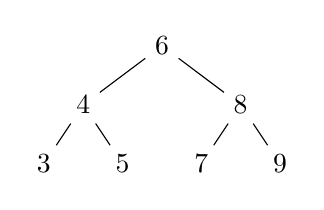
\begin{tikzpicture}[scale=0.5,
  level 1/.style={sibling distance=40mm},
  level 2/.style={sibling distance=20mm}]
\node{6}
	child{node{4}
		child{node{3}}
		child{node{5}}}
	child{node{8}
		child{node{7}}
		child{node{9}}};
\end{tikzpicture}

\begin{itemize}
	\item Unvollständiger BTS:
\end{itemize}

\begin{tikzpicture}[scale=0.5,
  level 1/.style={sibling distance=40mm},
  level 2/.style={sibling distance=20mm}]
\node{6}
	child{node{4}
		child{node{3}
			child{node{1}}
			child[missing]}
		child{node{5}}}
	child{node{8}
		child{node{7}}
		child{node{9}}};
\end{tikzpicture}

\end{answer}

\item Beweisen Sie durch eine geeignete Induktion: In jedem vollständigen binären Suchbaum ist die Anzahl der Blätter genau um eins größer als die Anzahl der inneren Knoten.

\begin{answer}
\begin{itemize}
	\item n jedem vollständigem BTS gilt: jeder Knoten n hat 0 oder genau 2 Kindknoten. 
    \item innerer Knoten: jeder Knoten v gilt als innerer Knoten gdw. v min. 1 Kindknoten hat.
    \item Blätter Knoten: Jeder Knoten v gilt als Blatt, wenn v keine Kinderknoten hat.
\end{itemize}

\textbf{Annahme:} In jedem vollständigen binären Suchbaum ist die Anzahl der Blätter genau um eins größer als die Anzahl der inneren Knoten. \\

base-case BTS mit einem inneren Knoten (root): \\
Angenommen der BTS erfüllt die Bedingungen eines vollständigen BTS und die Werte der Knoten spielen keine Rolle, dann muss gelten:  \\
$num_{\text{Blätter}}=num_{\text{innerer Knoten}}+1$


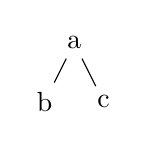
\begin{tikzpicture}[scale=0.5]
\node{a}
	child{node{b}}
	child{node{c}};
\end{tikzpicture}

Da die Werte in diesem Fall unerheblich sind, gilt die Zeichnung für einen vollständingen BTS mit einem inneren Knoten: \\
\begin{itemize}
	\item $num_{\text{innerer Knoten}}=a \text{ } num_{\text{innere Knoten}}=1$ 
	\item $num_{\text{Blätter}}=b,c \text{ } num_{\text{Blätter}}=2$ 
\end{itemize}

Die Anahme gilt im base-case. \\

\textbf{I.S:} Wenn die Annahme bei n inneren Knoten gilt, gilt sie auch $n+1$ inneren Knoten. 
Ein vollständiger BTS mit n inneren Knoten erfüllt die Gleichung:  \\
$num_{\text{Blätter}} = num_{\text{innerer Knoten}} + 1$ \\
Wenn es einen inneren Knoten zusätzlich geben soll, wird ein Blattknoten zu diesem Knoten und bekommt nach der Definition von vollständigen BTS 2 neue Kindknoten, da:

\begin{enumerate}
	\item nur 1 Kind Widerspruch mit Definition von vollständigen BTS.
	\item 0 Kindknoten, dann bleibt $num_{\text{innerer Knoten}}$ gleich, da das Blatt nicht zum Inneren Knoten werden konnte.
\end{enumerate}

\end{answer}


\item Formulieren Sie eine ähnliche Aussage für allgemeine binäre Suchbäume und beweisen Sie sie.
\end{enumerate}

\newpage
\section*{{Problem 1: Elementare Wahrscheinlichkeitsrechnung}}

Auf einem Tisch stehen $N$ Kisten. In diese Kisten werden nacheinander unabhängig voneinander $n$ Bälle geworfen, wobei jede Kiste mit gleicher Wahrscheinlichkeit getroffen wird.\\

\begin{enumerate}
\item[a)] Berechnen Sie die Wahrscheinlichkeit, dass Kiste i leer ist. Sei Yi die Zufalls-
variable, die den Wert 1 annimmt, falls Kiste i leer ist, und 0 sonst. Geben Sie
auch den Erwartungswert E[Yi ] an.\\
Hinweis: Wenn Kiste $i$ leer bleibt, dann landen alle $n$ Bälle in den $N - 1$ anderen Kisten.\\

\textbf{Lösung:}\\

Wahrscheinlichkeit, dass bei $n$ unabgängigen Ballwürfen eine von $N$ Kisten $i$ leer ist.\\
$Pr(\text{Ball landet in Kiste } i ) = (1 \text{ over N})$\\
$Pr(overline\{ \text{Ball landet in Kiste }i\}) = ((N-1) \text{ over N})$\\
Es wird betrachtet, dass $Pr(overline\{ \text{Ball landet in Kiste }i\})$ $n-mal$ hintereinander eintritt.\\
Für die Wahrscheinlichkeit, dass Eine Kisten $i$ nach $n$ unabhängigen Würfen leer ist gilt:\\
$Pr(\text{Kiste i ist nach n Versuchen leer}) = Pr_1(overline\{ \text{Ball landet in Kiste }i\}) *$ \\ $\text{        }Pr_2(overline\{ \text{Ball landet in Kiste }i\}) *...* Pr_n(overline\{ \text{Ball landet in Kiste }i\})$\\
$Pr(\text{Kiste i ist nach n Versuchen leer}) = ((N-1)$ $over$ $N) * ((N-1)$ $over$ $N) *...* ((N-1)$ $over$ $N)$  $(n*mal)$\\
$Pr(\text{Kiste i ist nach n Versuchen leer}) = ((N-1)$ $over$ $N)^n$\\

\noindent
Für die Zufallsvariable $Y_i$ gilt:\\
$Y_i = 1$ gdw. Kiste $i$ ist leer $\rightarrow$ Kiste $i$ ist nach $n$ unabhängigen Versuchen leer.\\
$Y_i = 0$ gdw. Kiste $i$ ist nicht leer.\\

\noindent
$E(Y_i)$ Für den Erwartungswert wird $Y_i$ als Bernouli-Zufallsvariable betrachtet. daher gilt:\\
$E(Y_i) = 0*(1-p)+1*p$\\ 
$p = ((N-1) over N)^n$\\
$E(Y_i) = 0*(1-p) + 1* ((N-1)$ $over$ $N)^n$\\


\item[b)] Sei $X$ die Zufallsvariable, welche die Anzahl von leeren Kisten angibt. Berechnen Sie den Erwartungswert von $X$ mit Hilfe der Erwartungswerte $E[Yi]$.\\

\textbf{Lösung:}\\
$X = Y_1 + Y_2 + ... + Y_n$ (Die Summe aller $Y_i$, dass alle Kisten leer sind. Gleichverteilung) $Y_i = 1$, wenn die Kiste leer ist, $Y_i = 0$, wenn sie nicht leer ist.\\
$E[X] = N*E[Y_i]$\\
$E[X] = N*((N-1) over N)^n$\\

\item[c)] Bestimmen Sie, wie viele Bälle man benötigt, damit gilt: mit Wahrscheinlichkeit mindestens 1/2 enthält mindestens eine Kiste mindestens zwei Bälle.\\ 
$Hinweis:$ Stellen Sie sich vor, die $n$ Bälle werden nacheinander in die Kisten
geworfen. Was ist die Wahrscheinlichkeit, dass der nächste Ball in einer leeren Kiste landet, wenn alle vorherigen Bälle in einer leeren Kiste gelandet sind? Verwenden Sie die ungemein nützliche Abschätzung $1 + x \leq e^x$ , welche für alle $x \in R$ gilt.\\

\textbf{Lösung:}\\
Sei das Ergebnis, dass alle $n$ Bälle in verschiedene Kisten fallen. Jeder Kiste hat höchstens 1 Ball $E$. ges: $n -> Pr(E) <= 1$ over $2$\\
Wahrscheinlichkeit, dass ein Ball in eine Kiste $i$ fällt $Pr(\omega_1) = (1$ over $N)$\\
Wahrscheinlichkeit, dass ein 2. Ball in eine Kiste $j, j <> i$ fällt $Pr(\omega_2) = ((N-1)$ over $N)$\\
Wahrscheinlichkeit, dass ein 3. Ball in eine leere Kiste $l$ fällt, $Pr(\omega_3) = ((N-2)$ over $N)$
Wahrscheinlichkeit, dass ein $n$. Ball in eine leere Kiste fällt, $Pr(\omega_n) = ((N-(n-1))$ over $N)$\\

\item[d)] Professor Pinocchio hat eine Idee, um Hashtabellen zu vereinfachen. Wenn
wir die Zahl $N$ der Plätze in der Hashtabelle im Verhältnis zur Anzahl der zu
speichernden Einträge $n$ groß genug wählen, sollte die Wahrscheinlichkeit, dass
Kollisionen auftreten, verschwindend gering werden (unter der Annahme, dass
sich die Hashfunktion wie eine zufällige Funktion verhält). Dann könnte man
auf die Kollisionsbehandlung verzichten. In Anbetracht von (c), was halten Sie
von dem Vorschlag? (Wenn Sie Teil (c) nicht gelöst haben, dann bearbeiten Sie
diesen Teil unter der Annahme, dass für $N^{1/3}$ Bälle mindestens eine Kollision
auftritt.\\

\textbf{Lösung:}\\
Meiner Meinung nach ist es nie gut, Fehlerbehandlung, in diesem Fall Kollisionsbehandlung, wegzulassen. Solange die Wahrscheinlichkeit nicht $0.00\%$ liegt, sollte Fehlerbehandlung weiterhin unterstützt werden, da es in diesem Fehlerfall zu kritischen Fehlern im Programm oder System führen kann. Zusätzlich Wir haben in $c)$ gesehen, dass die maximale Wahrscheinlichkeit, dass Bälle (hier Einträge) jedes Mal in einem anderen Slot zugeordnet werden, bei einem zufälligen Wurf/Treffer (beim Hashen Zuweisung) $50:50$ beträgt. Das ist meiner Meinung nach nicht ausreichend, um Kollisionsbehandlung wegzulassen. Daher würde ich dem Professor widersprechen.

\end{enumerate}



\newpage

\newpage
\pbitem{Binäre Suchbäume}
\begin{enumerate}
\item Angenommen, wir haben einen binären Suchbaum T , welcher die Zahlen von
1 bis 1000 als Schlüssel speichert. Wir suchen in T nach dem Schlüssel 363.
Bestimmen Sie für jede der folgenden Schlüsselfolgen, ob sie als Folge der
Einträge auf dem Suchpfad nach 363 auftreten kann. Begründen Sie jeweils
Ihre Antwort.


\begin{enumerate}
\item \textbf{2, 252, 401, 398, 330, 344, 397, 363.}

\begin{answer}
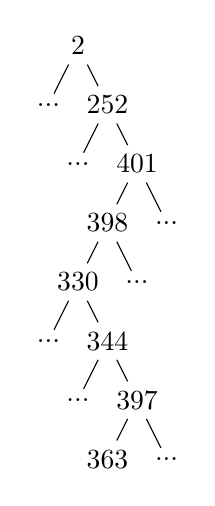
\begin{tikzpicture}[scale=0.5]

\node {2}
	child{node{...}}
	child{ node{252}
		child{node{...}}
		child{node {401}
			child{node{398}
				child{node{330}
					child{node{...}}
					child{node{344}
						child{node{...}}
						child{node{397}
							child{node{363}}
							child{node{...}}}}}
				child{node{...}}}
			child{node{...}}}};
\end{tikzpicture}

\begin{center}
\small
\hspace*{-3cm}
\begin{tabular}{@{} c c l c c @{}}
\toprule
\textbf{Schritt} & \textbf{Aktueller Knoten} & \textbf{Vergleich mit Ziel 363} & \textbf{Nächster Schritt} & \textbf{Intervall für nächsten Knoten} \\
\midrule
1 & 2   & \( 363 > 2 \Rightarrow \) rechts & 252 & \([3, 1000]\) \\
2 & 252 & \( 363 > 252 \Rightarrow \) rechts & 401 & \([253, 1000]\) \\
3 & 401 & \( 363 < 401 \Rightarrow \) links & 398 & \([253, 400]\) \\
4 & 398 & \( 363 < 398 \Rightarrow \) links & 330 & \([253, 397]\) \\
5 & 330 & \( 363 > 330 \Rightarrow \) rechts & 344 & \([331, 397]\) \\
6 & 344 & \( 363 > 344 \Rightarrow \) rechts & 397 & \([345, 397]\) \\
7 & 397 & \( 363 < 397 \Rightarrow \) links & 363 & \([345, 396]\) \\
8 & 363 & Ziel erreicht & — & — \\
\bottomrule
\end{tabular}
\end{center}

\end{answer}

\item \textbf{924, 220, 911, 244, 898, 258, 362, 363.}

\begin{answer}
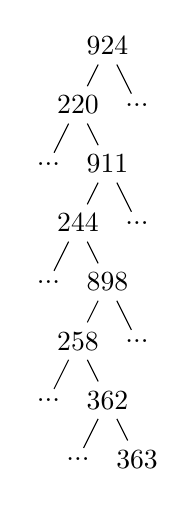
\begin{tikzpicture}[scale=0.5]
\node{924}
	child{node{220}
		child{node{...}}
		child{node{911}
			child{node{244}
				child{node{...}}
				child{node{898}
					child{node{258}
						child{node{...}}
						child{node{362}
							child{node{...}}
							child{node{363}}}}
					child{node{...}}}}
			child{node{...}}}}
	child{node{...}};
\end{tikzpicture}

\begin{center}
\small
\hspace*{-3cm}
\begin{tabular}{@{} c c l c c @{}}
\toprule
\textbf{Schritt} & \textbf{Aktueller Knoten} & \textbf{Vergleich mit Ziel 363} & \textbf{Nächster Schritt} & \textbf{Intervall für nächsten Knoten} \\
\midrule
1 & 924 & \( 363 < 924 \Rightarrow \) links & 220 & \([1, 923]\) \\
2 & 220 & \( 363 > 220 \Rightarrow \) rechts & 911 & \([221, 923]\) \\
3 & 911 & \( 363 < 911 \Rightarrow \) links & 244 & \([221, 910]\) \\
4 & 244 & \( 363 > 244 \Rightarrow \) rechts & 898 & \([245, 910]\) \\
5 & 898 & \( 363 < 898 \Rightarrow \) links & 258 & \([245, 897]\) \\
6 & 258 & \( 363 > 258 \Rightarrow \) rechts & 362 & \([259, 897]\) \\
7 & 362 & \( 363 > 362 \Rightarrow \) rechts & 363 & \([363, 897]\) \\
8 & 363 & Ziel erreicht & — & — \\
\bottomrule
\end{tabular}
\end{center}

\end{answer}


\item \textbf{925, 202, 911, 240, 912, 245, 363.}

\begin{answer}
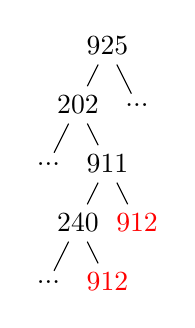
\begin{tikzpicture}[scale=0.5]
\node{925}
	child{node{202}
		child{node{...}}
		child{node{911}
			child{node{240}
				child{node{...}}
				child{node{\textcolor{red}{912}}}}
			child{node{\textcolor{red}{912}}}}}
	child{node{...}};
\end{tikzpicture}

\begin{center}
\small
\hspace*{-3cm}
\begin{tabular}{@{} c c l c c @{}}
\toprule
\textbf{Schritt} & \textbf{Aktueller Knoten} & \textbf{Vergleich mit Ziel 363} & \textbf{Nächster Schritt} & \textbf{Intervall für nächsten Knoten} \\
\midrule
1 & 925 & \( 363 < 925 \Rightarrow \) links & 202 & \([1, 924]\) \\
2 & 202 & \( 363 > 202 \Rightarrow \) rechts & 911 & \([203, 924]\) \\
3 & 911 & \( 363 < 911 \Rightarrow \) links & 240 & \([203, 910]\) \\
4 & 240 & \( 363 > 240 \Rightarrow \) rechts & 912 & \([241, 910]\) \\
5 & 912 & \( 363 < 912 \Rightarrow \) links & & \textcolor{red}{\( 912 > [910] \Rightarrow \) Fehler} \\
\bottomrule
\end{tabular}
\end{center}

\begin{itemize}
	\item Der Knoten 912 liegt nicht mehr im Intervall von [241,910] und somit ist der Knoten nicht in der \textbf{Schlüsselfolge}.
\end{itemize}
\end{answer}

\item \textbf{2, 399, 387, 219, 266, 382, 381, 278, 363.}

\begin{answer}
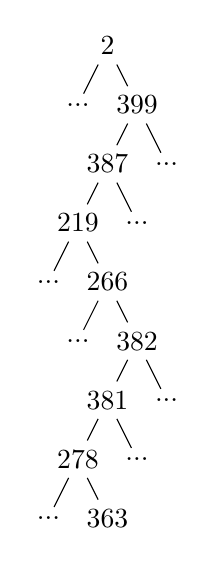
\begin{tikzpicture}[scale=0.5]
\node{2}
	child{node{...}}
	child{node{399}
		child{node{387}
			child{node{219}
				child{node{...}}
				child{node{266}
					child{node{...}}
					child{node{382}
						child{node{381}
							child{node{278}
								child{node{...}}
								child{node{363}}}
							child{node{...}}}
						child{node{...}}}}}
			child{node{...}}}
		child{node{...}}};
\end{tikzpicture}

\begin{center}
\small
\hspace*{-3cm}
\begin{tabular}{@{} c c l c c @{}}
\toprule
\textbf{Schritt} & \textbf{Aktueller Knoten} & \textbf{Vergleich mit Ziel 363} & \textbf{Nächster Schritt} & \textbf{Intervall für nächsten Knoten} \\
\midrule
1 & 2 & \( 363 > 2 \Rightarrow \) rechts & 399 & \([3, 1000]\) \\
2 & 399 & \( 363 < 399 \Rightarrow \) links & 387 & \([3, 398]\) \\
3 & 387 & \( 363 < 387 \Rightarrow \) links & 219 & \([3, 386]\) \\
4 & 219 & \( 363 > 219 \Rightarrow \) rechts & 266 & \([220, 386]\) \\
5 & 266 & \( 363 > 266 \Rightarrow \) rechts & 382 & \([267, 386]\) \\
6 & 382 & \( 363 < 382 \Rightarrow \) links & 381 & \([267, 381]\) \\
7 & 381 & \( 363 < 381 \Rightarrow \) links & 278 & \([267, 380]\) \\
8 & 278 & \( 363 > 278 \Rightarrow \) rechts & 363 & \([279, 380]\) \\
9 & 363 & Ziel Erreicht! & - & - \\
\bottomrule
\end{tabular}
\end{center}

\end{answer}

\item \textbf{935, 278, 347, 621, 299, 392, 358, 363.}

\begin{answer}
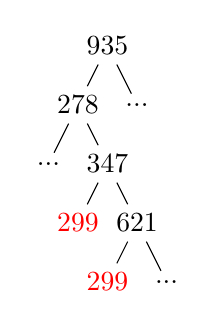
\begin{tikzpicture}[scale=0.5]
\node{935}
	child{node{278}
		child{node{...}}
		child{node{347}
			child{node{\textcolor{red}{299}}}
			child{node{621}
				child{node{\textcolor{red}{299}}}
				child{node{...}}}}}
	child{node{...}};
\end{tikzpicture}

\begin{center}
\small
\hspace*{-3cm}
\begin{tabular}{@{} c c l c c @{}}
\toprule
\textbf{Schritt} & \textbf{Aktueller Knoten} & \textbf{Vergleich mit Ziel 363} & \textbf{Nächster Schritt} & \textbf{Intervall für nächsten Knoten} \\
\midrule
1 & 935 & \( 363 < 935 \Rightarrow \) links & 278 & \([1, 934]\) \\
2 & 278 & \( 363 > 278 \Rightarrow \) rechts & 347 & \([279, 934]\) \\
3 & 347 & \( 363 > 347 \Rightarrow \) rechts & 621 & \([348, 934]\) \\
4 & 621 & \( 363 < 621 \Rightarrow \) links & 299 & \([348, 620]\) \\
5 & 299 & \( 363 > 299 \Rightarrow \) rechts & & \textcolor{red}{\( 299 < [348] \Rightarrow \) Fehler} \\
\bottomrule
\end{tabular}
\end{center}

\begin{itemize}
	\item Der Knoten 299 liegt nicht mehr im Intervall von [348,620] und somit ist der Knoten nicht in der \textbf{Schlüsselfolge}.
\end{itemize}

\end{answer}

\end{enumerate}

\item Sei T ein binärer Baum mit n Knoten, und sei K eine total geordnete Menge
von n Schlüsseln. Zeigen Sie, dass es genau eine Möglichkeit gibt, die Schlüssel
aus K auf die Knoten von T zu verteilen, so dass die binäre Suchbaumeigen-
schaft erfüllt ist.
\end{enumerate}


\pbitem{AVL-Bäume}
\begin{enumerate}
\item Fügen Sie die Schlüssel A, L, G, O, D, T, S, X, Y, Z in dieser Reihenfolge in
einen anfangs leeren AVL-Baum ein. Löschen Sie sodann die Schlüssel Z, A,
L. Zeichnen Sie den Baum nach jedem Einfüge- und Löschvorgang, und zeigen
Sie die Rotationen, welche durchgeführt werden. Annotieren Sie dabei auch
die Knoten mit ihrer jeweiligen Höhe.

\item Beweisen Sie: Beim Einfügen in einen AVL-Baum wird höchstens eine (Einfach-
oder Doppel-)Rotation ausgeführt. Gilt das auch beim Löschen (Begründung)?
\end{enumerate}


	
	
	
\end{problemlist}

%Quellen Reference
%\newpage
%\printbibliography

\end{document}